\documentclass[xcolor={dvipsnames},handout]{beamer}

\usepackage{assets/pres-template_MOW}
\usepackage{pdfpages}

%--------------------------------------------------------------------------
% Specific to this document ---------------------------------------
%--------------------------------------------------------------------------
% \setbeamercovered{transparent}

%%%%%%%%%%%%%%%%%%%%%%%%%%%%%%%%%%%
\setlength{\tabcolsep}{1.3pt}
\title{PLSC 48110/28110}
\subtitle{Lecture 4: Experiments and covariate adjustment}
\date{}
\author{Molly Offer-Westort}
\institute{Department of Political Science, \\University of Chicago}
\IfFileExists{upquote.sty}{\usepackage{upquote}}{}
\hypersetup{pdftitle={PLSC 48110/28110 - Lecture 4: Experiments and covariate adjustment},pdfauthor={Molly Offer-Westort},pdfpagemode=UseNone}
\begin{document}

%-------------------------------------------------------------------------------%
\frame{\titlepage
\thispagestyle{empty}
}
%-------------------------------------------------------------------------------%
\begin{frame}{Notation: recall}

\begin{itemize}
\item Dependent variable: ($Y$), the thing we want to study variation in; also ``outcome'', ``response''. 
\item Independent variable: ($W$) in causal settings, the thing that we manipulate. Also ``treatment.''
\item In non-causal settings, something that may have some natural variation in the population associated with the dependent variable ($X$). 
\end{itemize}
\end{frame}


%%%%%NOTE%%%%%
\note{
\scriptsize \singlespacing

\begin{itemize}
\item xxxx
\end{itemize}

}

%-------------------------------------------------------------------------------%
\begin{frame}{Potential outcomes: notation}

$W$ is binary. 
$$
Y_i^{obs} = \begin{cases}
Y_i(0) & W_i = 0 \\
Y_i(1) & W_i = 1 \\
\end{cases}
$$

\end{frame}


%%%%%NOTE%%%%%
\note{
\scriptsize \singlespacing

\begin{itemize}
\item xxxx
\end{itemize}

}

%-------------------------------------------------------------------------------%
\begin{frame}{Estimand of interest: ATE}


\begin{itemize}
\item Individual treatment effect
$$
\tau_i = Y_i(1)-Y_i(0)
$$ 
\item Average treatment effect
$$
\tau = \E[\tau_i]  = \E[Y_i(1)-Y_i(0)]
$$

\item We're interested in the \textit{average} difference in potential outcomes had we applied treatment $W$, vs. if we had not. 
\end{itemize}

\end{frame}



%%%%%NOTE%%%%%
\note{
\scriptsize \singlespacing

\begin{itemize}
\item xxxx
\end{itemize}

}

%-------------------------------------------------------------------------------%
\begin{frame}{Difference-in-means}

Proposed estimator for $\E[\tau_i]$: compare people who received treatment $1$ to people who received treatment $0$. \\~\


This is the difference in means estimator:

\begin{align*}
\hat\tau_{DM} & = \frac{\sum_i^n Y_i^{obs} W_i}{\sum_i^n W_i} - \frac{\sum_i^n Y_i^{obs} (1-W_i)}{\sum_i^n (1-W_i)}\\
& = \bar Y^{obs}_t - \bar Y^{obs}_c\nonumber
\end{align*}

\end{frame}


%%%%%NOTE%%%%%
\note{
\scriptsize \singlespacing

\begin{itemize}
\item xxxx
\end{itemize}

}

%-------------------------------------------------------------------------------%
\begin{frame}{Regression version of this}

\[
Y_i^{obs} = \alpha + \tau \cdot W_i + \varepsilon_i
\]

$\varepsilon_i$ is an unobserved error term.

The ``ordinary least squares'' (OLS) regression solution is
\begin{align*}
\hat\tau_{ols} & = \frac{\sum_{i = 1}^n (W_i - \bar W ) \cdot (Y_i^{obs} - \bar Y^{obs}) }{\sum_{i = 1}^n (W_i - \bar W )^2} = \bar Y^{obs}_t - \bar{Y}^{obs}_c\\
\hat \alpha_{ols} & = \bar Y^{obs} - \hat \tau_{ols} \cdot \bar W
\end{align*}


This estimate is equivalent to the difference-in-means estimate (check this). 

\end{frame}


%%%%%NOTE%%%%%
\note{
\scriptsize \singlespacing

\begin{itemize}
\item xxxx
\end{itemize}

}

%-------------------------------------------------------------------------------%
\begin{frame}{Inference}

\begin{itemize}
\item ``randomization implies that the average residuals for treated and control units are zero''
\item $\E[\varepsilon_i \rvert W_i = 0] = 0$ and $\E[\varepsilon_i \rvert W_i = 1] = 0$
\item But random assignment does not imply errors are independent of $W_i$  (what does this mean?)  
\item[$\rightarrow$] estimate with ``robust'' standard errors 
\end{itemize}

\end{frame}


%%%%%NOTE%%%%%
\note{
\scriptsize \singlespacing

\begin{itemize}
\item ``the error term has a clear meaning as the difference between potential outcomes and their population expectation, rather than as the difference between the realized outcome and its conditional expecta- tion given the treatment. Moreover, the independence of Wi and [Yi(0),Yi(1)], directly implied by the randomization, now has implications for the properties of the error term.''
\end{itemize}

}

%-------------------------------------------------------------------------------%
\begin{frame}{Estimation}
Using the \cite{duflo2012incentives} data,
\begin{gather}
\begin{aligned}
\hat Y_{i}^{obs} & = & 0.5805 & \quad + & 0.2145 & \cdot W_i,&&\\
& & (0.0356) & & (0.0308) \\
& & & &  [0.0311]\nonumber
\end{aligned}
\end{gather}

where $Y$ is teacher attendance and $W$ is assignment to the monitoring and financial-incentive program.

\end{frame}


%%%%%NOTE%%%%%
\note{
\scriptsize \singlespacing

\begin{itemize}
\item xxxx
\end{itemize}

}

%-------------------------------------------------------------------------------%
\begin{frame}{Why adjust for covariates?}

\begin{itemize}
\item improve precision  (when covariates correlate with the outcome)
\item assess heterogeneity 
\item account for imbalance in randomization 
\end{itemize}

\end{frame}


%%%%%NOTE%%%%%
\note{
\scriptsize \singlespacing

\begin{itemize}
\item xxxx
\end{itemize}

}

%-------------------------------------------------------------------------------%
\begin{frame}{Balance checks}

\cite{olken2010direct} Table 2

\centering
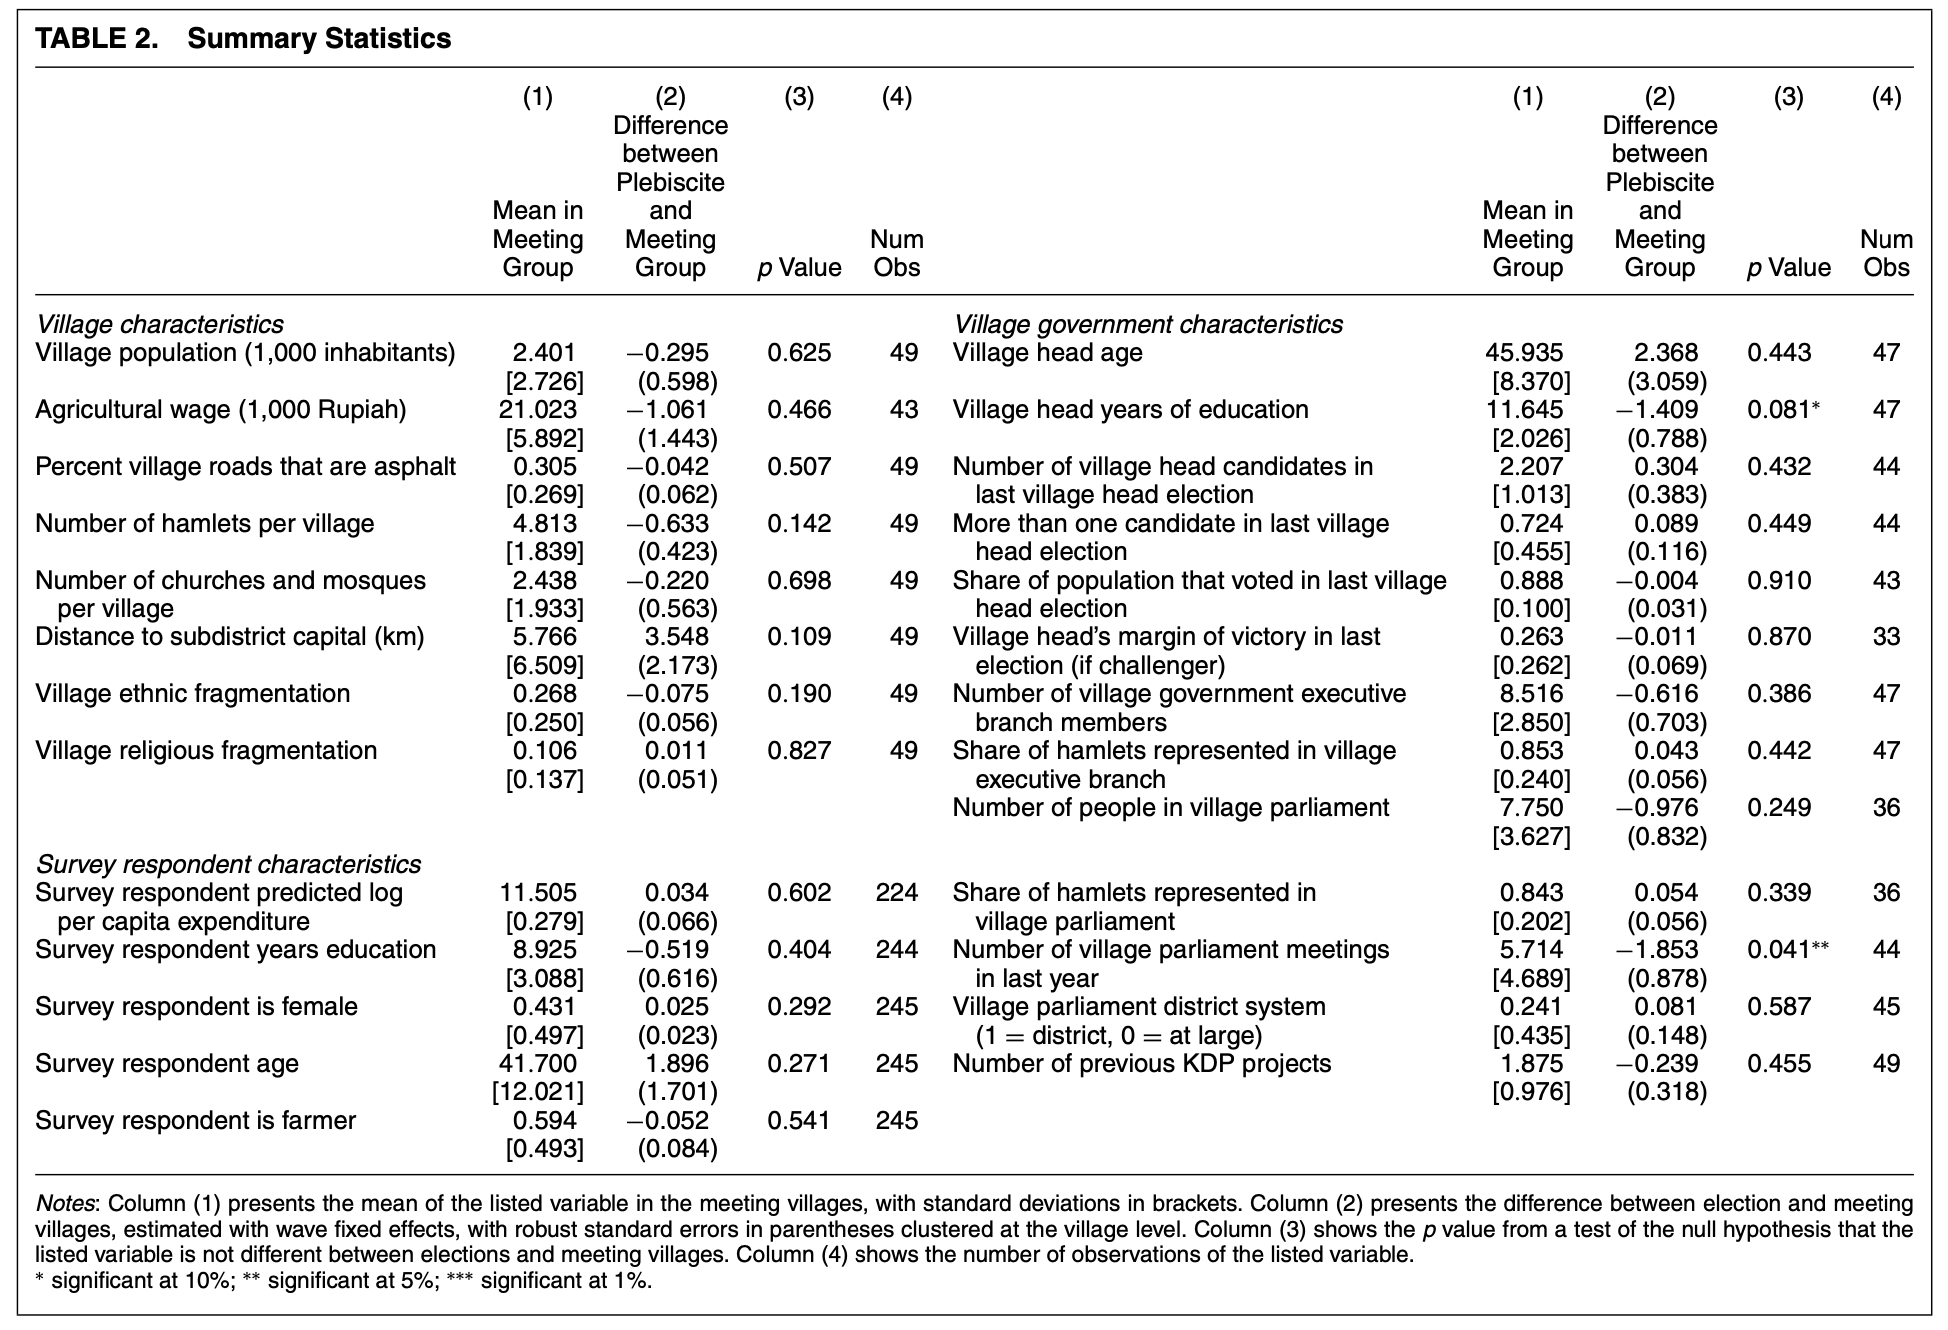
\includegraphics[width=\textwidth,height=0.72\textheight,keepaspectratio]{assets/olken_2010_T2.png}

\end{frame}


%%%%%NOTE%%%%%
\note{
\scriptsize \singlespacing

\begin{itemize}
\item xxxx
\end{itemize}

}

%-------------------------------------------------------------------------------%
\begin{frame}{Estimation: using covariates additively}

\begin{gather}
\begin{aligned}
\hat Y_{i}^{obs} & = &\alpha + \tau \cdot W_i + \beta ' \dot X_i + \epsilon_i
\nonumber
\end{aligned}
\end{gather}

\begin{itemize}
\item $\dot X_i = X_i - \bar X$
\item Using covariate deviations mean that the interpretation of $\tau$ and $\beta$ does not change, just intercept $\alpha$. 
\end{itemize}

\end{frame}


%%%%%NOTE%%%%%
\note{
\scriptsize \singlespacing

\begin{itemize}
\item xxxx
\end{itemize}

}

%-------------------------------------------------------------------------------%
\begin{frame}{What is the issue with regression adjustment for experiments?}

\begin{itemize}
\item If covariates don't correlate well with the outcome, or 
\item If there are too many covariates relative to sample size, 
\item Adjustment can result in noisier estimates, inconsistent SE estimation, finite sample bias. 
\item Also: fishing. 
\end{itemize}

\end{frame}


%%%%%NOTE%%%%%
\note{
\scriptsize \singlespacing

\begin{itemize}
\item xxxx
\end{itemize}

}

%-------------------------------------------------------------------------------%
\begin{frame}{Addressing concerns}

\cite{lin2013agnostic}'s proposed estimator
\begin{itemize}
\item Separate regressions of $Y$ on $X$ in both treatment and control. 
\item Use robust SEs. 
\item Using treatment $\times$ covariate interactions resolves risks to precision, even under model mispecification. 
\item Small sample bias—how much should we care about it?
\end{itemize}

\end{frame}


%%%%%NOTE%%%%%
\note{
\scriptsize \singlespacing

\begin{itemize}
\item xxxx
\end{itemize}

}

%-------------------------------------------------------------------------------%
\begin{frame}{Using covariates with full interactions}

\begin{gather}
\begin{aligned}
\hat Y_{i}^{obs} & = &\alpha + \tau \cdot W_i + \beta ' \dot X_i + \gamma ' \dot X_i \cdot W_i+  \epsilon_i
\nonumber
\end{aligned}
\end{gather}

\begin{itemize}
\item In general, $\gamma$ don't have straightforward interpretation as differences in average treatment effects 
\item \textit{Unless} all covariates are indicators and can be used to partition the population.  
\end{itemize}

\end{frame}


%%%%%NOTE%%%%%
\note{
\scriptsize \singlespacing

\begin{itemize}
\item xxxx
\end{itemize}

}

%-------------------------------------------------------------------------------%
\begin{frame}{Interpretation with covariates}
Using the \cite{duflo2012incentives} data,
\begin{align*}
\hat Y_i^{obs}
  &= \underset{(0.02)}{0.59}
   + \underset{(0.03)}{0.192}\, W_i
   + \underset{(0.002)}{0.001}\, X_{1i}
   - \underset{(0.01)}{0.004}\, X_{2i} \\
  &\quad - \underset{(0.003)}{0.006}\, X_{1i}W_i
   + \underset{(0.01)}{0.017}\, X_{2i}W_i .
\end{align*}
where $X_1$, $X_2$ are covariates.
\end{frame}


%%%%%NOTE%%%%%
\note{
\scriptsize \singlespacing

\begin{itemize}
\item xxxx
\end{itemize}

}

%-------------------------------------------------------------------------------%
\begin{frame}{Rules of thumb with covariates}

\begin{itemize}
\item Pre-specify what you will measure and your main analyses. 
\item Don't include too many covariates relative to sample size. 
\item Checking covariate balance ex-post can be useful; but focus on using design decisions ex-ante to avoid great imbalance on measured variables
\item Use simpler forms of estimation: difference in means, stratified analysis, with robust SEs. 
\end{itemize}

\end{frame}


%%%%%NOTE%%%%%
\note{
\scriptsize \singlespacing

\begin{itemize}
\item xxxx
\end{itemize}

}

%-------------------------------------------------------------------------------%
\begin{frame}{Stratified analysis}
Using the \cite{duflo2012incentives} data,
\begin{align*}
\hat Y_i^{obs}
  &= \underset{(0.02)}{0.60}
   + \underset{(0.03)}{0.188}\, W_i
   + \underset{(0.05)}{0.010}\, 1_{X_{1i}>37} \\
  &\quad - \underset{(0.06)}{0.06}\, 1_{X_{1i}>37}W_i .
\end{align*}
where $X_1$ is teacher score.
\end{frame}


%%%%%NOTE%%%%%
\note{
\scriptsize \singlespacing

\begin{itemize}
\item xxxx
\end{itemize}

}

%-------------------------------------------------------------------------------%
\begin{frame}{Alternatives with machine learning methods}

\begin{itemize}
\item Flexibly model response. 
\item Accounting for large numbers of covariates. 
\item Substitution estimators; estimation of heterogeneous treatment effects. 
\item Role of pre-registration when analysis decisions are data driven?
\end{itemize}

\end{frame}


%%%%%NOTE%%%%%
\note{
\scriptsize \singlespacing

\begin{itemize}
\item xxxx
\end{itemize}

}

%-------------------------------------------------------------------------------%
\backupbegin
%-------------------------------------------------------------------------------%

\begin{frame}[allowframebreaks]{References}
    \bibliographystyle{apalike}
    \bibliography{assets/bib}
\end{frame}
%-------------------------------------------------------------------------------%
\backupend
\end{document}
